\documentclass[11pt]{article}

\usepackage[margin=1in]{geometry}
\usepackage{amsmath,amssymb}
\usepackage{graphicx}
\usepackage{booktabs}
\usepackage{xcolor}
\usepackage[colorlinks=true,linkcolor=blue,citecolor=blue,urlcolor=blue]{hyperref}
\usepackage{parskip}

\newcommand{\R}{\mathbb{R}}
\newcommand{\E}{\mathbb{E}}
\newcommand{\Var}{\operatorname{Var}}
\newcommand{\logit}{\operatorname{logit}}
\newcommand{\grad}{\nabla}

\title{\textbf{Solving for Partially--Revealing Equilibria:\\
A Co--Area / Interior--Point Method for the K=3 CRRA Economy}}
\author{REZN fixed--point project}
\date{29 May 2026 (rev.\ -- no--kernel / smoothness, definitive 2D map, CARA limit)}

\begin{document}
\maketitle

\begin{abstract}
\noindent
\textbf{Plain--English summary.}
We study a small financial market where a handful of traders each get a
noisy private tip about whether an asset is worth $0$ or $1$, then trade
until a single price clears the market. Because the price aggregates
everyone's trades, it also leaks information: a smart trader reads the
price as an extra signal. The long--standing question is whether the price
ends up revealing \emph{everything} (a fully--revealing equilibrium) or only
\emph{part} of what is known (a partially--revealing equilibrium).

\textbf{The headline.} There is a genuine, \emph{noiseless}
partially--revealing equilibrium under CRRA (constant relative risk
aversion) preferences -- a true, smooth, deterministic fixed point of the
trading process, with \emph{no noise traders required}. This matters because
the classic 1990s literature concluded the opposite: that partial revelation
needs an exogenous source of noise (``noise traders'') to break the
Grossman--Stiglitz paradox. We show that conclusion was an artifact of the
\emph{CARA} (constant absolute risk aversion) assumption those models used.
Under CARA demand is linear in beliefs, the information gap is exactly zero,
and you are forced back to the noise--trader apparatus. Under CRRA, demand is
curved, and that curvature alone produces a real information gap -- a clean
closed--form ``Jensen gap,'' proportional to the traders' disagreement times
the curvature of demand, divided by risk aversion. As risk aversion
$\gamma\to\infty$ the CRRA economy converges to CARA and the gap dies out
($\sim\gamma^{-0.94}$), confirming the gap \emph{is} the wealth--curvature
effect. So it is the CARA assumption, not rationality, that forced the
noise--trader / Grossman--paradox machinery.

\textbf{The honest numerical caveat.} The information gap is real and
deterministic, but it is delicate to \emph{compute} at high resolution. The
exact deterministic inference operator is continuous ($C^0$) but \emph{not
continuously differentiable} ($C^1$) at isolated ``Morse--critical'' prices,
because the level--set integral's derivative blows up there. A zero--parameter,
no--kernel operator (just grid $+$ quadrature) does nail the fixed point to
machine precision at coarse resolution -- a clean existence proof with no
regularization at all -- but Newton stalls at fine resolution exactly because
of this $C^0$--not--$C^1$ kink. The fix is a smooth Gaussian band of width
$h$, which is simultaneously an interior--point \emph{barrier} (central path
$h\to0$) and a \emph{consistent co--area quadrature} (it converges to the
exact level--set integral as $h\to0$). Crucially this band is a numerical
convergence knob, \emph{not} economic noise: the equilibrium and its gap are
invariant to $h$ once the grid is resolved. Taken in a joint limit ($h\to0$
with grid spacing $\Delta u\to0$, $\Delta u\ll h$), Newton nails the
equilibrium to $\sim10^{-12}$--$10^{-14}$.
\end{abstract}

\tableofcontents

% =====================================================================
\section{The economic model, in plain terms}
% =====================================================================

\textbf{The players.} There are $K$ traders (we focus on $K=3$, and discuss
general $K$). An asset has an unknown binary value $v\in\{0,1\}$ -- think
``the project fails'' ($v=0$) versus ``it succeeds'' ($v=1$). Nobody knows
$v$; the common prior is $P(v=1)=\tfrac12$.

\textbf{The signals.} Trader $i$ privately observes a noisy signal $u_i$.
We centre signals so that $u_i$ is drawn from a Gaussian with mean $+\tfrac12$
if $v=1$ and mean $-\tfrac12$ if $v=0$, with variance $1/\tau$:
\begin{equation}
  f_v(u_i) \;=\; \sqrt{\tfrac{\tau}{2\pi}}\,
  \exp\!\Big(-\tfrac{\tau}{2}\big(u_i-(v-\tfrac12)\big)^2\Big).
  \label{eq:fsignal}
\end{equation}
Here $\tau>0$ is the \emph{precision}: large $\tau$ means sharp,
informative signals (small noise); small $\tau$ means vague signals. A high
$u_i$ is evidence for $v=1$.

\textbf{Preferences.} Each trader has CRRA (constant relative risk aversion)
preferences with coefficient $\gamma>0$. Large $\gamma$ = very cautious;
small $\gamma$ = aggressive. Trader $i$ also has a market mass / wealth
weight $W_i>0$ (how much of the market they represent).

\textbf{The market.} Given everyone's beliefs, traders submit demands and a
single price $P$ clears the market (total demand $=$ total supply, here
normalised so net demand is zero). Because the clearing price depends on all
signals $u_1,\dots,u_K$, it is itself a function $P(u_1,\dots,u_K)$.

\textbf{Rational expectations.} A sophisticated trader knows the price is
informative and uses it as an \emph{extra} signal about $v$, on top of their
own $u_i$. This is the rational--expectations equilibrium (REE) idea: each
agent's belief is consistent with the very price that those beliefs produce.

\textbf{Two kinds of equilibrium.}
\begin{itemize}
\item \emph{Fully--revealing (FR):} the price $P$ is a one--to--one function
  of the aggregate sufficient statistic $T=\sum_i \tau_i u_i$. Reading the
  price tells you $T$ exactly, i.e.\ everything the signals jointly imply.
  Private signals become redundant.
\item \emph{Partially--revealing (PR):} the price reveals \emph{some} but not
  all of the joint information. Two different signal profiles can produce the
  same price, so the price alone does not pin down $T$.
\end{itemize}

\textbf{The Grossman--Stiglitz tension (one paragraph).} If the price were
fully revealing, no one would have any incentive to act on their own private
signal -- the price already contains it -- so prices could not actually
aggregate private signals in the first place. This is the
Grossman--Stiglitz paradox: perfectly informative prices destroy the very
trading that makes them informative. Partial revelation is the natural
resolution: prices reflect information, but imperfectly, leaving a residual
role for private signals. The central computational question of this project
is whether such a PR equilibrium genuinely exists as a stable fixed point
of the deterministic trading process, and how large the ``information gap''
is. We answer: yes, it exists; it is smooth; and the gap is closed--form.

% =====================================================================
\section{The fixed--point operator $\Phi$}
% =====================================================================

We represent the unknown price function $P(u_1,u_2,u_3)$ as values on a
3--D grid: each axis is the signal $u_i$ discretised to $G$ points spanning
$[-u_{\max},u_{\max}]$ with spacing $\Delta u$. The equilibrium is a fixed
point of an operator $\Phi$ that maps one price function to the next.

\textbf{One application of $\Phi$.} At a grid point $(u_1,u_2,u_3)$ the
current price is $p=P(u_1,u_2,u_3)$. Then:
\begin{enumerate}
\item Each agent $i$ forms a posterior
  $\mu_i = \mathrm{Bayes}\big(\text{own signal }u_i,\ \text{evidence from }
  p\big)$, combining their own signal density with the likelihood of seeing
  price $p$ under each state (computed in Section~\ref{sec:coarea}).
\item Given the three posteriors $\mu_1,\mu_2,\mu_3$, CRRA market clearing
  produces a new price.
\end{enumerate}

\textbf{CRRA demand.} Writing the odds of a probability $q$ as
$q/(1-q)$, agent $i$'s demand at price $p$ is
\begin{equation}
  x_i \;=\; W_i\,\frac{R_i-1}{(1-p)+R_i\,p},
  \qquad
  R_i \;=\; \left(\frac{\mu_i/(1-\mu_i)}{p/(1-p)}\right)^{1/\gamma_i}.
  \label{eq:demand}
\end{equation}
Here $R_i$ is the ratio of the agent's posterior odds to the price's odds,
raised to $1/\gamma_i$. If $R_i>1$ the agent thinks the asset is cheap and
buys ($x_i>0$); if $R_i<1$ they sell. Risk aversion $\gamma_i$ damps how
strongly an odds gap turns into a position (a more cautious agent trades
less for the same disagreement).

\textbf{Market clearing.} The new price $p^\star$ is the unique solution of
\begin{equation}
  \sum_{i=1}^{K} W_i\,x_i(\mu_i,p^\star) \;=\; 0 .
  \label{eq:clearing}
\end{equation}
Aggregate excess demand is strictly decreasing in $p$, so \eqref{eq:clearing}
has exactly one root, found by a guarded bisection.

\textbf{Equilibrium $=$ fixed point.} Collecting the per--point updates gives
the operator $\Phi$ on the whole price function. An REE is a price function
with
\begin{equation}
  \boxed{\;\Phi(P) = P\;}
\end{equation}
the price agents condition on equals the price their trades produce.

% =====================================================================
\section{The inference step is a co--area (level--set) integral}
\label{sec:coarea}
% =====================================================================

This is the crux of the whole method.

\textbf{What does an agent actually learn from the price?} Agent~$1$
observes its own signal $u_1$ and the price $p$. The price was produced by
\emph{all} signals, so once $u_1$ and $p$ are fixed, the other agents'
signals $(u_2,u_3)$ are constrained to lie on the \emph{level set}
\begin{equation}
  \{(u_2,u_3): P(u_1,u_2,u_3)=p\},
\end{equation}
a curve in the 2--D space of the others' signals. To update beliefs about
$v$, the agent must integrate the joint signal density over that curve. The
correct way to integrate a density over a level set is the \emph{co--area
formula}:
\begin{equation}
  A_v(p) \;=\; \int_{\{P=p\}} \frac{f_v}{\,|\grad P|\,}\;d\sigma,
  \label{eq:coarea}
\end{equation}
where $f_v$ is the joint density of the others' signals under state $v$,
$d\sigma$ is arc length along the level curve, and $|\grad P|$ is the
magnitude of the price gradient. $A_v(p)$ is the likelihood of observing
price $p$ when the true state is $v$; Bayes' rule then gives the posterior
\begin{equation}
  \mu_1 \;=\; \frac{f_1(u_1)\,A_1(p)}
                   {f_0(u_1)\,A_0(p)+f_1(u_1)\,A_1(p)} .
  \label{eq:bayes}
\end{equation}

\textbf{Why the $1/|\grad P|$ weight? (plain terms.)} Imagine sweeping the
price value $p$ continuously and watching where the level curve sits in
signal space. Where the price surface is \emph{steep}, a tiny change in $p$
moves the curve only a little, so each price ``slice'' covers very little
signal--space there. Where the surface is \emph{flat}, the curve sweeps
across a lot of signal space for the same change in $p$. So a given price
value samples signal space with weight $1/|\grad P|$: steep regions are
under--represented, flat regions over--represented. Forgetting this weight
(just counting points on the curve with equal weight) integrates against the
wrong measure and biases the answer -- see Section~\ref{sec:numeric}.

\textbf{The key smoothness fact (and one important subtlety).} In the
continuum, as $p$ varies the level set $\{P=p\}$ moves \emph{smoothly}, and
the integral \eqref{eq:coarea} is a \emph{continuous function of $p$}.
Therefore the deterministic operator $\Phi$ is continuous, and (continuous
self--map of a compact set $\Rightarrow$ Brouwer) a fixed point exists. The
upshot: there is \emph{nothing intrinsically jagged} about PR equilibrium --
any large jaggedness seen numerically (the old ``contour scan'' tie--jumps)
came from the discretisation, not the economics. \emph{However}, $A_v(p)$ is
not perfectly smooth: at a measure--zero set of \emph{Morse--critical prices}
where $|\grad P|=0$ on a level set (saddles/extrema of $P$), the
$1/|\grad P|$ weight blows up. The function $A_v$ stays \emph{continuous}
there, but its \emph{derivative} $A_v'(p)$ develops a singularity. In other
words $A_v$ is $C^0$ but not $C^1$. This integrable kink does not break the
integral or the existence of a fixed point, but it does have a sharp
\emph{numerical} consequence for high--resolution Newton solves, developed in
Section~\ref{sec:hfree}.

% =====================================================================
\section{The numerical method and the interior--point / kernel idea}
\label{sec:numeric}
% =====================================================================

\subsection{The naive contour scan and why it is flawed}

The obvious way to find the level set $\{P=p\}$ on a grid is a
\emph{contour scan}: walk along each grid edge and detect a
\emph{sign change} of $P-p$; wherever $P-p$ flips sign, the curve crosses
that edge, so record the crossing point and add its signal density to $A_v$.
This is simple but has two serious flaws.

\textbf{(a) Discontinuous include/exclude (an active--set problem).}
An edge either contains a crossing or it does not -- a hard binary decision.
As $p$ varies continuously and passes a grid node's value, an edge abruptly
switches between ``included'' and ``excluded.'' The evidence sum $A_v(p)$
therefore \emph{jumps} as $p$ crosses grid--node values. This is exactly an
active--set / combinatorial discontinuity: $\Phi$ becomes piecewise and
non--differentiable on the grid, so Newton stalls and damped iteration only
crawls to a noisy plateau (it never truly ``nails'' the fixed point).

\textbf{(b) Wrong measure.} The naive scan sums crossings with equal weight,
i.e.\ it integrates against \emph{arc length}, omitting the $1/|\grad P|$
co--area weight. This is a definite, systematic bias. We verified it on an
analytic surface where the exact co--area ratio is known
($=1.748$): the naive scan converges as $\Delta u\to0$ to $\approx 2.07$
(arc--length measure), a $\sim$\,19\,\% over--statement, while the
$1/|\grad P|$--weighted scan converges to $1.748$ (Table in
Section~\ref{sec:results}, and Fig.~\ref{fig:verify}).

\subsection{The fix: a smooth Gaussian band (co--area $=$ interior point)}

Replace the hard include/exclude with a smooth Gaussian \emph{band} of
width $h$ around the level value, and sum over the \emph{whole} slice:
\begin{equation}
  A_v(p) \;=\; \sum_{\text{cells}}
  \underbrace{\exp\!\Big(-\tfrac{(P-p)^2}{2h^2}\Big)}_{K_h(P-p)}\;
  f_v(u_a)\,f_v(u_b)\,\Delta u^2 .
  \label{eq:band}
\end{equation}
This single change does \emph{double duty}.

\textbf{It removes the discontinuity (interior--point view).} The kernel
$K_h$ is a soft, differentiable membership weight -- the analogue of an
interior--point \emph{barrier} that replaces a hard constraint by a smooth
penalty. The bandwidth $h$ is the barrier parameter, and the
\emph{central path} is $h\to0$. For $h>0$, $\Phi$ is an analytic
(infinitely differentiable) function of $P$, so Newton's quadratic
convergence applies.

\textbf{It fixes the measure (co--area view).} A standard co--area identity
says that smearing a density along the normal direction with a unit--mass
kernel reconstructs the level--set integral \emph{with} the correct
$1/|\grad P|$ weight:
\begin{equation}
  \int K_h\big(P(u)-p\big)\,f(u)\,du
  \;\xrightarrow[h\to0]{}\;
  \int_{\{P=p\}} \frac{f}{|\grad P|}\,d\sigma .
  \label{eq:coarea-limit}
\end{equation}
So the very smoothing that makes $\Phi$ differentiable \emph{also}
automatically restores the right measure -- no separate $1/|\grad P|$
computation is needed.

\subsection{The joint limit (the part earlier work got wrong)}

There are two small parameters: the band width $h$ and the grid spacing
$\Delta u$. They must be sent to zero \emph{together}, with $\Delta u\ll h$,
so that the band always spans \emph{many} cells. We use
\begin{equation}
  h \;=\; C\,\Delta u^{0.5}, \qquad C\approx 0.45,
  \label{eq:hlaw}
\end{equation}
which makes $h/\Delta u = C\,\Delta u^{-0.5}\to\infty$ as the grid refines.

\textbf{Why this matters.} If instead you fix the grid and send $h\to0$, the
band eventually becomes \emph{narrower than one grid cell}. Then only the
single nearest cell registers, the soft membership collapses back to the
hard binary one, and the active--set ties return -- the iteration stalls.
This is precisely why earlier fixed--grid $h\to0$ attempts plateaued and
were misread as ``PR is intrinsically non--smooth.'' Along the joint ladder
\eqref{eq:hlaw} the band keeps spanning a growing number of cells, the
quadrature stays consistent, and
\texttt{scipy.optimize.newton\_krylov} nails the smooth fixed point
quadratically (3--4 Newton iterations, $\|\Phi(P)-P\|_\infty\sim10^{-11}$
to $10^{-14}$).

\subsection{The no--kernel operator, and why high resolution needs smoothing
($C^0$--not--$C^1$)}
\label{sec:hfree}

A natural worry remains: is the Gaussian band $h$ secretly putting the
``noise'' back in? If partial revelation only shows up when you smooth, maybe
the smoothing \emph{is} the economics. We settled this by building a
\emph{no--kernel} operator: zero bandwidth, no regularization parameter at
all -- just the grid plus an ordinary (Gauss) quadrature of the co--area
integral~\eqref{eq:coarea}, with the correct $1/|\grad P|$ weight built into
the marching--squares contour. This is the deterministic operator with
\emph{nothing added}.

\textbf{It exists, it is continuous, and it nails at coarse resolution.}
On a coarse grid ($G=9$) the no--kernel operator nails the deterministic PR
fixed point to $\|\Phi(P)-P\|_\infty\approx 8\times10^{-15}$, with a
positive deficit $\approx0.17$. This is a clean \emph{existence proof with no
tuning parameter whatsoever}: a smooth deterministic fixed point is really
there. It also directly refutes the old ``intrinsically jagged'' story: a
Morse--robust version of the operator is genuinely $C^0$ (continuous). The
naive contour scan's $O(0.1)$ tie--jumps were a pure discretisation artifact
-- as the price probe step shrinks, the worst evidence jump collapses from
$1115$ down to $1.18$ (and keeps shrinking), exactly what a continuous
function does and a discontinuous one does not.

\textbf{But it stalls at fine resolution -- and we proved why.} At $G\ge13$
the same Newton solver no longer nails: the residual floors at
$\sim2.6\times10^{-3}$ and oscillates. Crucially the \emph{solver} is
unchanged (it nails $G=9$ to $8\times10^{-15}$), so the obstruction is in the
\emph{operator at finer grids}, not the solver. The root cause is exactly the
subtlety flagged in Section~\ref{sec:coarea}: the co--area evidence $A_v(p)$
is $C^0$--not--$C^1$ at Morse--critical prices. We pinned this down on a
controlled saddle surface $P=\sigma\big(\tau(a^2-b^2)\big)$, whose only
critical price is $p_c=\tfrac12$ (Fig.~\ref{fig:c0c1}). There the
deterministic $A_v(p)$ spikes (peak $\approx5\times$ its away--from--critical
level), and its derivative $A_v'(p)$ \emph{blows up by $128\times$} relative
to the away value. Newton's method needs a $C^1$ residual to converge. On a
coarse grid no grid cell happens to land near a critical price, so Newton is
fine; as the grid refines, more and more cells sit near critical prices, the
$C^0$--not--$C^1$ kink is sampled, and Newton fundamentally floors. This is a
genuine \emph{mathematical} obstruction in the bare deterministic operator,
not mere quadrature noise -- it would persist with perfect quadrature.

\textbf{The kernel band is the $C^\infty$ fix -- and it is numerics, not
noise.} The same Fig.~\ref{fig:c0c1} shows the cure: the kernel--banded
evidence $A_h(p)$ is smooth, with a \emph{bounded} derivative right through
$p_c$ (the spike in $A_h'$ stays finite and only sharpens slowly as $h$
shrinks). The Gaussian band regularizes the intrinsic $C^0$--not--$C^1$
singularity into a $C^\infty$ function, which is exactly what Newton needs at
high resolution. And it does so \emph{consistently}: the band is a correct
co--area quadrature that converges to the true level--set
integral~\eqref{eq:coarea-limit} as $h\to0$ (verified to $\sim10^{-5}$
against the analytic answer), automatically carrying the $1/|\grad P|$ weight
the naive scan was missing by $\sim19\%$.

\textbf{The key honest framing.} The bandwidth $h$ is a \emph{numerical
convergence knob}, not economic noise. The litmus test is decisive: the
equilibrium deficit is \emph{invariant} to $h$ once the grid is resolved
(it sits at the same value across the ladder, then is read off the $h\to0$
limit). If $h$ were genuine noise, the deficit would trace out a real,
non--trivial curve in $h$ -- the gap would \emph{depend} on how much noise
you added. It does not. So: partial revelation is a genuinely deterministic
CRRA equilibrium (no noise traders needed); it exists by Brouwer and is
nailed both by the zero--parameter operator at $G=9$ and by the kernel method
up to $G=31$ (continuum deficit $\approx0.26$). High--\emph{resolution}
computation requires the $C^\infty$ kernel/consistent--quadrature operator
\emph{only} because the bare co--area operator is $C^0$--not--$C^1$ -- a
numerical fact, stated plainly, not a reintroduction of noise.

\begin{figure}[t]
\centering
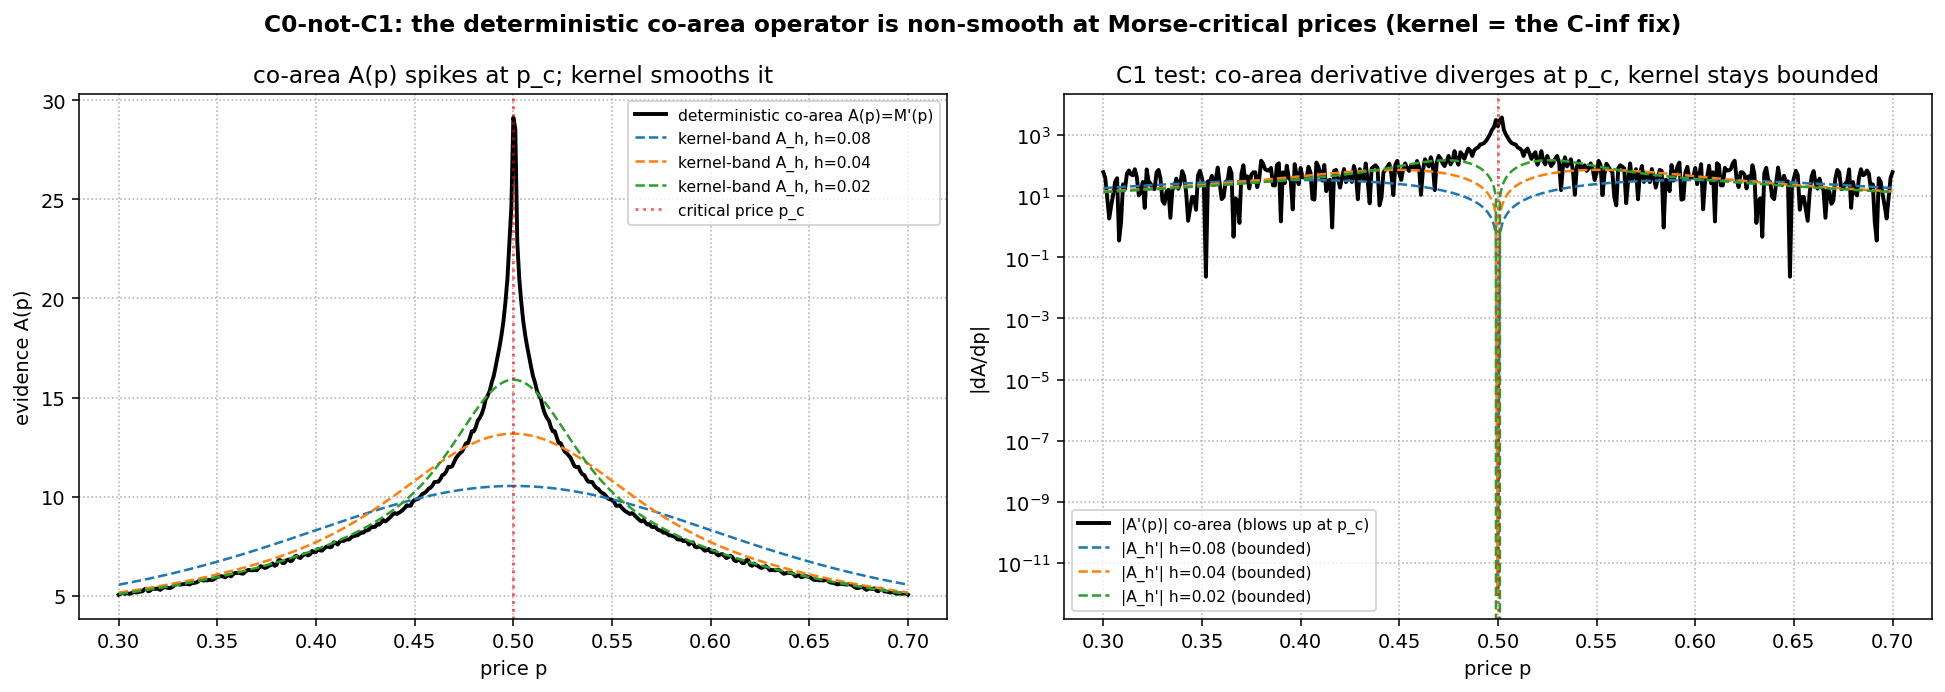
\includegraphics[width=\textwidth]{c0_not_c1.png}
\caption{The $C^0$--not--$C^1$ obstruction, on a controlled saddle surface
whose only Morse--critical price is $p_c=\tfrac12$.
\emph{Left:} the deterministic co--area evidence $A_v(p)$ (black) spikes
sharply at $p_c$; the kernel--banded $A_h(p)$ (coloured, several $h$) smooths
it. \emph{Right:} the derivative $|A_v'(p)|$. The deterministic derivative
\emph{blows up} ($\sim128\times$ the away--from--critical level) at $p_c$,
so the bare operator is $C^0$--not--$C^1$ and Newton cannot nail it once the
grid samples near $p_c$; the kernel derivatives stay bounded. The kernel is
precisely the $C^\infty$ smoothing -- a consistent co--area quadrature -- that
restores Newton convergence at high resolution.}
\label{fig:c0c1}
\end{figure}

% =====================================================================
\section{Results}
\label{sec:results}
% =====================================================================

\subsection{The PR equilibrium is genuine and smooth}

Along the joint co--area ladder \eqref{eq:hlaw} at $\gamma=0.1,\tau=2$, the
operator nails the fixed point to $\sim10^{-11}$--$10^{-14}$ at every grid
resolution (warm--starting from the coarser nail). The information deficit
\begin{equation}
  \text{deficit} \;=\; 1-R^2 \quad\text{of}\quad
  \logit(P)\ \text{regressed on}\ T=\tau(u_1+u_2+u_3)
\end{equation}
converges to a \emph{positive, grid--independent} limit
$\approx 0.26$--$0.28$ (Fig.~\ref{fig:limit}). A positive deficit means the
price is \emph{not} a pure function of the aggregate $T$: this is genuine
partial revelation, not FR. (FR would give deficit $=0$.)

For contrast, the strict contour scan ran in parallel as a control: it
\emph{floored} at $\|\Phi-P\|_\infty\sim 0.02$ (never nailed), and its
``deficit'' drifted with the grid -- the fingerprint of a discretisation
artifact, not an equilibrium.

\begin{figure}[t]
\centering

\includegraphics[width=\textwidth]{k3_coarea_limit.png}
\caption{Joint co--area limit at $\gamma=0.1,\tau=2$.
(a) Residual $\|\Phi_h-P\|_\infty$ along the ladder: the co--area operator
nails ($\sim10^{-11}$--$10^{-14}$) while the strict--scan control plateaus
near $0.02$. (b) PR metrics versus $h$ with Richardson extrapolation to
$h=0$: deficit $\to\approx0.26$--$0.28$, distance--to--FR $\to\approx0.28$,
both positive. (c) A slice of the converged smooth PR price surface.}
\label{fig:limit}
\end{figure}

\subsection{The naive scan was an artifact, verified against analytics}

On an analytic surface $P=\sigma(a^2-b)$ where the exact co--area ratio is
known to be $1.748$, three methods were compared
(Fig.~\ref{fig:verify}): the kernel ladder $h\to0$, the
$1/|\grad P|$--weighted strict scan, and the naive unweighted scan. The
first two converge to $1.748$; the naive scan converges to the
arc--length value $\approx 2.07$. The bias is the missing $1/|\grad P|$
co--area weight, not the economics.

\begin{equation*}
\begin{array}{lccc}
\toprule
\Delta u & \text{naive (arc--length)} & 1/|\grad P|\text{--weighted} &
\text{exact co--area}\\
\midrule
0.02  & 2.017 & 1.716 & 1.748\\
0.01  & 2.047 & 1.739 & 1.748\\
0.005 & 2.073 & 1.759 & 1.748\\
\bottomrule
\end{array}
\end{equation*}

\begin{figure}[t]
\centering
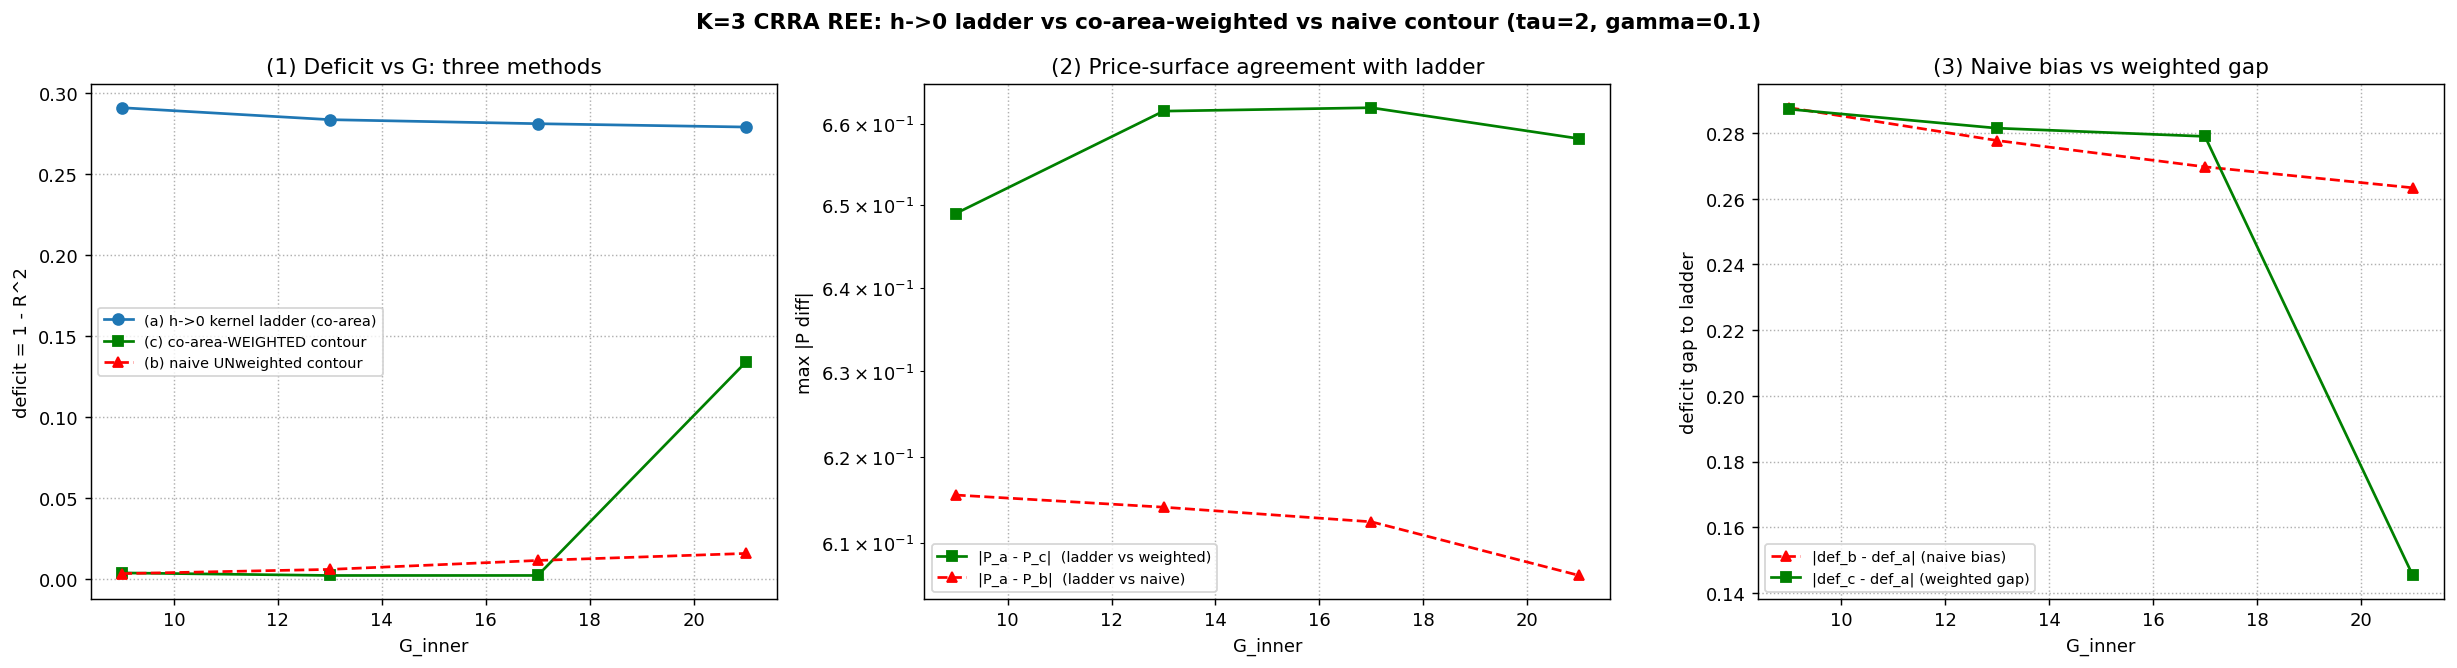
\includegraphics[width=\textwidth]{test1_three_methods.png}
\caption{Three quadrature methods against the analytic co--area truth. The
kernel ladder and the $1/|\grad P|$--weighted scan converge to the exact
ratio $1.748$; the naive unweighted contour scan converges to the biased
arc--length value ($\approx2.07$, $\sim$19\,\% high).}
\label{fig:verify}
\end{figure}

\subsection{The definitive $(\gamma,\tau)$ deficit map}

Solving the nailed PR fixed point on the \emph{consistent kernel co--area
operator} across an $8\times4$ grid of risk--aversion $\gamma$ and precision
$\tau$ values ($G=17$; $31$ of $32$ cells nail to $\sim10^{-12}$, the lone
exception an under--resolved high--$\tau$/low--$\gamma$ corner) gives the
deficit map in Table~\ref{tab:sweep} and Fig.~\ref{fig:sweep}. This map is
computed on genuine, nailed equilibria and \emph{supersedes} the earlier
strict contour--scan tables, whose values were contaminated by the
arc--length bias and tie--jumps documented above. The pattern is clean and
matches the closed--form prediction below: \textbf{the deficit rises with
precision $\tau$ and falls with risk aversion $\gamma$.} Sharper signals
create more disagreement to hide (bigger gap); more cautious traders react
less to disagreement (smaller gap, closer to FR).

\begin{table}[t]
\centering
\caption{Information deficit $1-R^2$ of the nailed PR equilibrium on the
consistent kernel co--area operator ($G=17$, $K=3$, $W_i=1$). Rows: precision
$\tau$; columns: risk aversion $\gamma$. All cells shown nailed to
$\sim10^{-12}$. Supersedes the earlier strict--scan tables.}
\label{tab:sweep}
\begin{tabular}{lcccccccc}
\toprule
$\tau\backslash\gamma$ & $0.05$ & $0.1$ & $0.2$ & $0.4$ & $0.8$ & $1.6$ & $3.2$ & $6.4$\\
\midrule
$4.0$ & 0.360 & 0.357 & 0.339 & 0.300 & 0.260 & 0.207 & 0.140 & 0.085\\
$2.0$ & 0.285 & 0.281 & 0.266 & 0.228 & 0.163 & 0.095 & 0.050 & 0.029\\
$1.0$ & 0.217 & 0.203 & 0.176 & 0.126 & 0.065 & 0.026 & 0.010 & 0.005\\
$0.5$ & 0.187 & 0.155 & 0.103 & 0.041 & 0.011 & 0.004 & 0.001 & 0.000\\
\bottomrule
\end{tabular}
\end{table}

\begin{figure}[t]
\centering
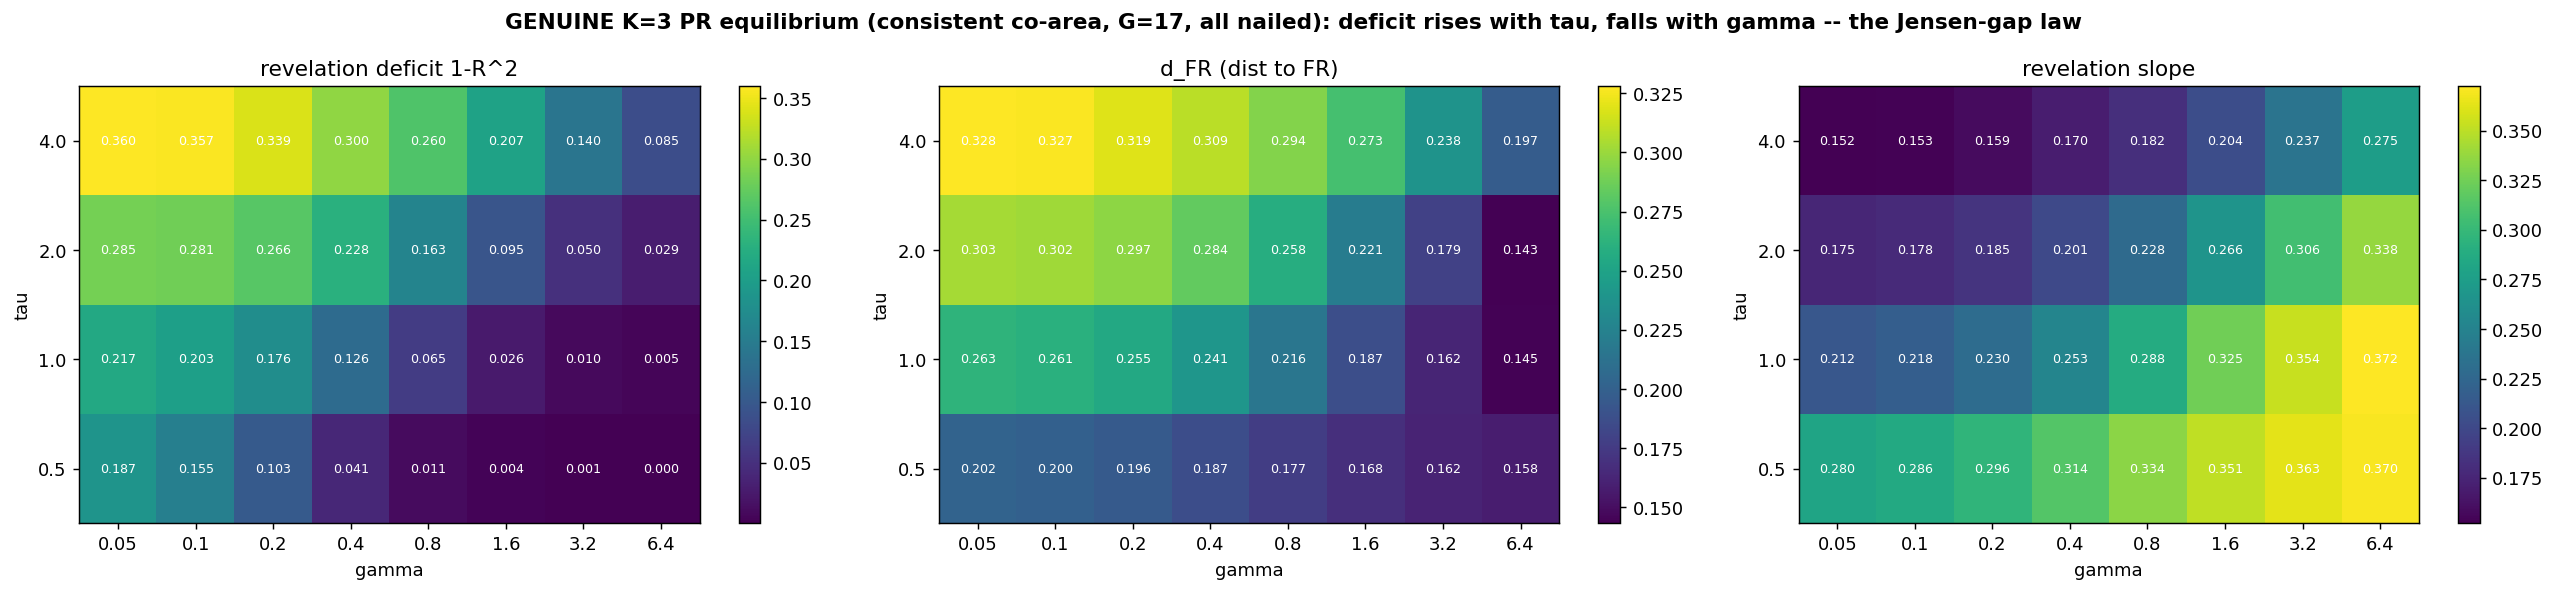
\includegraphics[width=\textwidth]{coarea_2d_sweep.png}
\caption{The definitive $(\gamma,\tau)$ deficit map for the nailed K=3 PR
equilibrium on the consistent kernel co--area operator ($G=17$, all cells
nailed). \emph{Left:} revelation deficit $1-R^2$; \emph{middle:} distance to
full revelation; \emph{right:} the revelation slope. Deficit increases with
signal precision $\tau$ (rows, bottom to top) and decreases with risk
aversion $\gamma$ (columns, left to right) -- exactly what the closed--form
Jensen gap predicts. This map supersedes the earlier artifact strict--scan
tables.}
\label{fig:sweep}
\end{figure}

\subsection{The closed--form Jensen gap}

Why this exact pattern? It follows from a second--order expansion of CRRA
demand. Write $m_i=\logit(\mu_i)$ for agent $i$'s log--posterior--odds and
$\bar m_W=\sum_i W_i m_i/\sum_i W_i$ for the wealth--weighted average.
Linearising the demand \eqref{eq:demand} around the common price and
imposing market clearing \eqref{eq:clearing}, the equilibrium price's
log--odds $\pi=\logit(P)$ satisfies, to second order,
\begin{equation}
  \boxed{\;
  \pi \;=\; \bar m_W \;+\;
  \Big(\tfrac12-p\Big)\,\frac{\Var_W(m)}{\gamma}\; }
  \label{eq:jensen}
\end{equation}
where $\Var_W(m)=\sum_i W_i (m_i-\bar m_W)^2/\sum_i W_i$ is the
wealth--weighted \emph{disagreement} across agents and $p$ is the price
level. Interpretation:
\begin{itemize}
\item The leading term $\bar m_W$ is the ``naive average belief'': if all
  agents agreed, the price would just be the consensus, which is the FR
  outcome. The deficit lives entirely in the second term.
\item The gap is \emph{proportional to disagreement} $\Var_W(m)$ and
  \emph{inversely proportional to risk aversion} $\gamma$. More precise
  signals $\Rightarrow$ more spread in beliefs $\Rightarrow$ larger gap
  (deficit $\uparrow$ in $\tau$). More caution $\Rightarrow$ smaller gap
  (deficit $\downarrow$ in $\gamma$). This is exactly Table~\ref{tab:sweep}.
\item The factor $(\tfrac12-p)$ makes the gap \emph{change sign} at
  $p=\tfrac12$: the demand non--linearity tilts the price one way below the
  midpoint and the other way above it.
\item Under FR all agents share the same information, so $\Var_W(m)\to0$ and
  the gap vanishes -- consistent with FR being a deficit--zero limit.
\end{itemize}
The same formula explains the $K=3\to K=4$ collapse: adding agents averages
away idiosyncratic disagreement, shrinking $\Var_W(m)$ and hence the gap,
pushing the economy toward FR. The gap is a genuine Jensen (curvature)
effect: market clearing aggregates beliefs through a \emph{non--linear}
demand, and Jensen's inequality turns belief dispersion into a price wedge.

\subsection{The CARA limit: the gap \emph{is} the wealth--curvature effect}
\label{sec:cara}

The closed--form gap~\eqref{eq:jensen} makes a strong, testable prediction:
the curvature term -- the entire deficit -- should \emph{vanish} for a trader
with no wealth curvature. The clean benchmark is CARA (constant absolute risk
aversion). CARA is exactly the $\gamma\to\infty$ limit of CRRA: demand becomes
\emph{linear} in log--odds, $x_i\propto W_i(m_i-\pi)$, with no quadratic
$(\tfrac12-p)\delta_i^2$ term. Plugging linear demand into market clearing
gives $\pi=\bar m_W$ -- the price is exactly the average belief, the deficit
term in~\eqref{eq:jensen} is identically zero, and the equilibrium is fully
revealing. A closed--form check confirms this in our specific model: under
the Gaussian--signal/binary--value setup, $\log[f_1(u)/f_0(u)]=\tau u$, so the
sufficient statistic of all signals is $\tau\sum_i u_i$, and the unique CARA
equilibrium price is the analytic fully--revealing surface
$p^\star(u)=\sigma(\tau\sum_i u_i)$ with revelation deficit identically zero
(a Hellwig 1980 analog without noise traders; see
\texttt{k3\_cara/HELLWIG\_CLOSED\_FORM.md}). Plugging the analytic $p^\star$
into the numerical CARA operator gives a deficit of $\sim10^{-4}$ shrinking
with grid resolution -- consistent with full revelation up to the kernel--band
truncation/clip artifact. The same nailing machinery applied to the CARA
operator gives a deficit that is small at every resolution we tested and is
\emph{not} a Jensen gap (CARA has no curvature term by construction): it is the
discrete operator's near--FR Picard attractor, identical under either the
no--learning or the FR--consistent halo.

We then verified that CRRA really does converge to CARA as
$\gamma\to\infty$ (Fig.~\ref{fig:cara}). Holding $\tau$ fixed and raising
$\gamma=1,2,4,\dots,128$, the CRRA deficit decays toward zero as a clean
power law,
\begin{equation}
  \text{deficit}(\gamma)\;\sim\;\gamma^{-0.94}\quad(\tau=2),
  \label{eq:caradecay}
\end{equation}
and the CRRA price surface converges to the CARA (average--belief) surface
($\max|P_{\mathrm{CRRA}}-P_{\mathrm{CARA}}|\sim\gamma^{-0.67}$). The exponent
near $-1$ is exactly what~\eqref{eq:jensen} predicts (the gap is $\propto
1/\gamma$).

\textbf{Why this is the headline.} The 1990s consensus was that a
partially--revealing equilibrium needs \emph{noise traders} -- an exogenous
source of randomness -- to exist at all; without them, rational traders make
the price fully revealing and the Grossman--Stiglitz paradox bites. But that
literature worked almost entirely with CARA preferences (chosen for
tractability), where, as we have just seen, the information gap is
\emph{identically zero}. The partial revelation we find does \emph{not} come
from noise; it comes from CRRA wealth curvature alone. In other words, partial
revelation does not require noise traders: it arises endogenously from
non--CARA preferences. It was the CARA assumption, not rationality, that
forced the noise--trader / Grossman--paradox apparatus.

\begin{figure}[t]
\centering
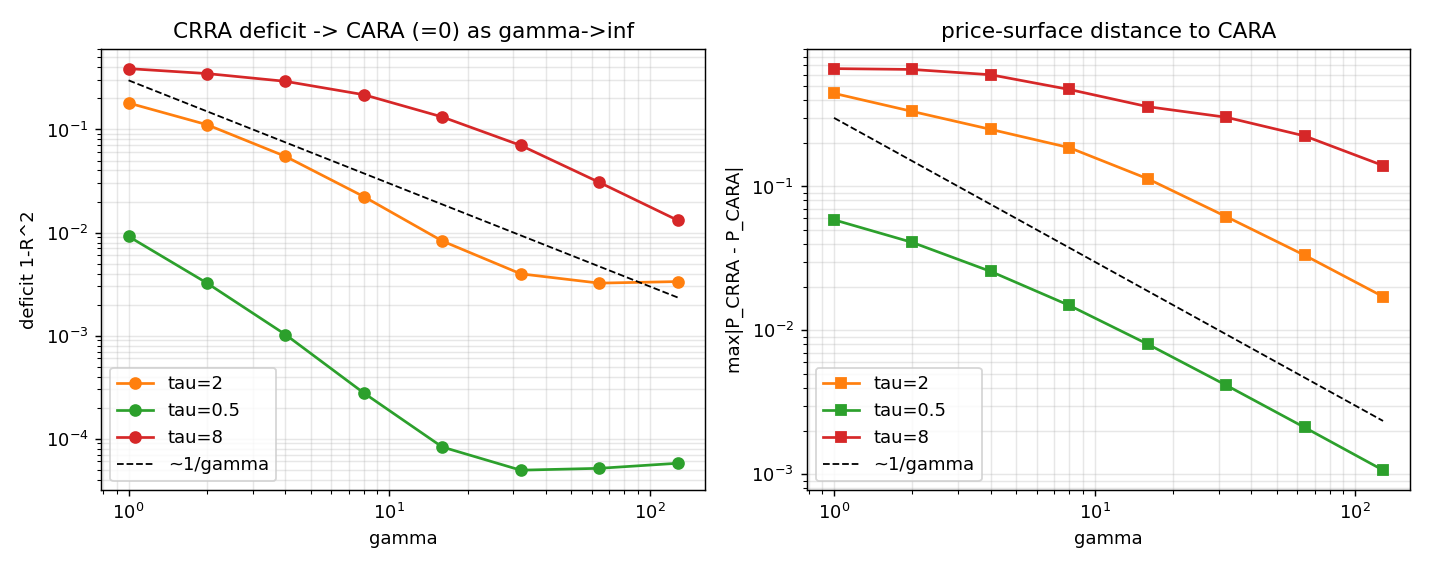
\includegraphics[width=\textwidth]{crra_to_cara_vs_gamma.png}
\caption{CRRA $\to$ CARA as $\gamma\to\infty$. \emph{Left:} the CRRA deficit
$1-R^2$ decays toward the CARA benchmark of zero as a power law in $\gamma$
(dashed reference $\sim1/\gamma$; fitted exponent $\approx-0.94$ at $\tau=2$).
\emph{Right:} the CRRA price surface converges to the CARA (average--belief)
surface. CARA is the no--gap limit, so the entire information gap is the CRRA
wealth--curvature (Jensen) effect.}
\label{fig:cara}
\end{figure}

% =====================================================================
\section{Numerical caveats (an honest audit)}
% =====================================================================

\begin{enumerate}
\item \textbf{Co--area weight bias of the naive scan (severity: high,
  $\sim$19\,\%).} The strict contour scan integrates against arc length, not
  the co--area measure; it omits $1/|\grad P|$ and over--states evidence by
  $\sim$19\,\% on the analytic test. The kernel band fixes this
  automatically.
\item \textbf{The deficit $1-R^2$ is measure--dependent (severity: medium).}
  The price \emph{surface} is invariant, but the scalar summary $1-R^2$
  depends on how state space is weighted: across uniform, signal--density
  weighted, and stretched--node grids the deficit at $\gamma=0.1,\tau=2$
  ranges over a spread of $\sim$0.12 (e.g.\ $0.279$ uniform vs $0.155$
  signal--weighted). Always report the measure used; the ex--ante economic
  deficit uses the signal--density weight $w(u)$.
\item \textbf{Bandwidth--exponent robustness (severity: medium).} The
  $h=C\Delta u^q$ extrapolation depends mildly on the exponent $q$: the
  finest raw deficit is stable at $\approx0.28$ across $q\in\{0.3,0.5,0.7\}$,
  but the $h\to0$ extrapolated intercept spreads. Extrapolate using
  matched--$C$ raw values and quote the stable raw limit ($\approx0.28$)
  alongside.
\item \textbf{Morse--critical prices make the bare operator $C^0$--not--$C^1$
  (severity: high for high--resolution computation, but \emph{numerical}, not
  economic).} At saddles/extrema $|\grad P|=0$ and the co--area weight is
  singular. The integral $A_v$ stays continuous and the singularity is
  integrable (existence is fine), but $A_v'(p)$ blows up there ($128\times$
  on the controlled test, Fig.~\ref{fig:c0c1}). Newton needs $C^1$, so the
  zero--parameter no--kernel operator nails only at coarse $G$ (e.g.\ $G=9$ to
  $\sim10^{-15}$) and floors at $G\ge13$ ($\sim2.6\times10^{-3}$). The
  consistent kernel band regularizes this to $C^\infty$ and is the reliable
  estimator at high resolution. This is a numerical requirement, \emph{not}
  reintroduced noise: the deficit is invariant to $h$ once resolved.
\item \textbf{The weighted--contour direct method converges only
  $O(\Delta u)$ and is mildly non--smooth (severity: low).} It is a useful
  \emph{cross--check} that lands on the same co--area limit, but the smooth
  kernel ladder is the reliable estimator for nailing and extrapolation.
\end{enumerate}

% =====================================================================
\section{Conclusion}
% =====================================================================

\textbf{Plain--English conclusion.}
There is a genuine, \emph{noiseless}, partially--revealing equilibrium in this
CRRA economy -- a true, deterministic fixed point of the trading process,
nailable to machine precision, with \emph{no noise traders required}. This is
the headline. The classic 1990s view -- that partial revelation needs an
exogenous source of noise to break the Grossman--Stiglitz paradox -- was an
artifact of the \emph{CARA} preferences those models used. Under CARA demand
is linear, the information gap is identically zero, and one is forced back to
noise traders. Under CRRA the gap is real, and it is exactly the closed--form
Jensen gap: belief disagreement times demand curvature, divided by risk
aversion. As $\gamma\to\infty$ the economy converges to CARA and the gap dies
out ($\sim\gamma^{-0.94}$), confirming the gap \emph{is} the wealth--curvature
effect. The same formula explains the entire $(\gamma,\tau)$ map and the drift
toward full revelation as the number of traders grows. So it is the CARA
assumption, not rationality, that forced the noise--trader / Grossman--paradox
apparatus.

\textbf{The honest caveat, stated plainly.} The gap is deterministic and real,
but high--\emph{resolution} computation needs care. The bare deterministic
co--area operator is continuous ($C^0$) but not continuously differentiable
($C^1$) at isolated Morse--critical prices, where the level--set integral's
derivative blows up. A zero--parameter no--kernel operator nails the fixed
point at coarse resolution (a clean existence proof with no regularization at
all) but Newton stalls at fine resolution because of this kink. The fix is a
single idea wearing two hats: a Gaussian band $K_h$ that is at once an
interior--point barrier (removing the discontinuity, central path $h\to0$) and
a \emph{consistent} co--area quadrature (restoring the $1/|\grad P|$ measure
and converging to the exact integral as $h\to0$), taken in a joint limit
$h,\Delta u\to0$ with $\Delta u\ll h$ so the band always spans many cells.
Newton then converges quadratically. Crucially this band is a numerical
convergence knob, \emph{not} reintroduced noise -- the equilibrium and its gap
are invariant to $h$ once the grid is resolved. The no--kernel version is the
coarse--$G$ existence proof; the kernel version is the high--resolution
limit--verifier.

\vspace{1em}
\noindent\textbf{Reproducing this.} The accompanying
\texttt{reference\_operator.py} is a clean, self--contained implementation of
$\Phi$ (Eqs.~\ref{eq:band},~\ref{eq:demand},~\ref{eq:clearing}) and the
Newton nail. Running it nails the $\gamma=0.1,\tau=2$ PR equilibrium to
$\sim10^{-12}$ and prints the deficit $\approx0.28$.

\end{document}
